\documentclass[letterpaper,12pt]{article}
\usepackage[left=1.25cm,right=1.25cm,top=2.25cm,bottom=2.25cm]{geometry}
\usepackage{amsmath, amsthm, amssymb}
\usepackage{verbatim}
\usepackage{hyperref}
\usepackage{color}
\usepackage{graphicx}
\usepackage{setspace}
\usepackage{natbib}

\usepackage{titlesec}
\setcounter{secnumdepth}{4}

\titleformat{\paragraph}
{\normalfont\normalsize\bfseries}{\theparagraph}{1em}{}
\titlespacing*{\paragraph}
{0pt}{3.25ex plus 1ex minus .2ex}{1.5ex plus .2ex}

% this command removes paragraph indentation and leaves a blank line between paragraphs.
% this looks better for a manual
\usepackage[parfill]{parskip}

%%% custom commands
%% for GPlates menus, selections etc. (\gp)
\newcommand{\gp}[1]{\textbf{#1}}

%% for terminal inputs (\tm)
\newcommand{\tm}[1]{\$ \texttt{#1}}

%% for terminal outputs (\tmo)
\newcommand{\tmo}[1]{\texttt{#1}}
%%% end of custom commands

%% Current GPlates models 
%% NOTE: be sure to sychronize these entries when the model is changed.
%% NOTE: also search this doc for instances of "2014" because some paths are directly referenced NOT using \gplatesmodel
%% NOTE include a blank space at the end 
\newcommand{\gplatesmodel}{Global\_Model\_WD\_Internal\_Release\_2014.1/ }
\newcommand{\gplatesmodelrot}{Global\_EarthByte\_TPW\_GeeK07\_2014.1.rot }

%% This is a convenient way to store case level sub dir names that may change
\newcommand{\caserecondir}{Reconstruction}

%%% for author notes
\newcommand{\mgnote}[1]{\textcolor{red}{MG: #1}}
\newcommand{\dbnote}[1]{\textcolor{blue}{DJB: #1}}
\newcommand{\nfnote}[1]{\textcolor{magenta}{NF: #1}}
\newcommand{\mtnote}[1]{\textcolor{cyan}{MT: #1}}
\newcommand{\tynote}[1]{\textcolor{green}{TY: #1}}

\begin{document}
\title{Creating 4-D Earth models using GPlates, CitcomS and the Geodynamic Framework}
\author{Michael Gurnis, Dan J. Bower, Mark Turner, Ting Yang\\
\small Seismological Laboratory, California Institute of Technology, Pasadena, CA 91125, USA\\
\small \texttt{gurnis@gps.caltech.edu, danb@gps.caltech.edu, mturner@gps.caltech.edu, tyang@gps.caltech.edu}
\and
Nicolas Flament, Rakib Hassan\\
\small Earthbyte Group, School of Geosciences, University of Sydney, NSW 2006, Australia\\
\small \texttt{nicolas.flament@sydney.edu.au, rakib.hassan@sydney.edu.au}
}
\date{\today}

\maketitle

% one half spacing is nice to read (uses setspace package)
\onehalfspacing

\tableofcontents

\listoffigures

\newpage


%%% SECTION 1 - INTRODUCTION %%%
\section{Introduction}
The purpose of this tutorial manual is to describe the workflows and data sets to create 4-D Earth models 
with GPlates, CitcomS, and the Geodynamic Framework (GDF).  
This manual assumes familiarity with GPlates, CitcomS, Python and Linux.  
The underlying concept of the 4-D models is that geophysical data, mostly from plate tectonic reconstructions, 
are assimilated into a time-dependent model of mantle convection.  
This data assimilation ensures that the convection model follows the geological constraints captured in the plate reconstructions.  
As such, the models are a hybrid between dynamic and kinematic approaches.  
The models are used to make predictions that can be tested with independent data, such as present day seismic structure, 
regional and global sea level, basin subsidence, heat flow, etc.

There are four aspects of the data assimilation.  
First, the 4-D simulations are forward models that start at some point in the past and are forward integrated in time to the present day.  
This means that the initial condition (IC) of the domain must be specified in terms of temperature, and if required, composition.  
Second, the models conform to a time-dependent velocity boundary condition.  
This velocity constraint on the top surface is specified as a Dirichlet boundary condition on the flow equation.  
The velocity boundary conditions can either arise from rigid plate models, or from models with deforming plates.  
Third, the models can conform to the evolving paleo age of the oceanic lithosphere (``lithosphere assimilation'').  
Fourth, the structure of subduction zones can conform to a simple thermal model of dipping subducted slabs (``slab assimilation'').  
The purpose of this last method is to ensure realistic asymmetric dipping subduction 
that otherwise can not be obtained with viscous flow, simple rheologies and kinematic boundary conditions.  
See \cite{BGF15} for a detailed explanation of our progressive data assimilation methods.

The assimilation procedure results in the creation of numerous files and directories over a series of steps.  We organize these steps into several main stages: 

\begin{itemize}
\item Preparing directories and input files with GPlates.
\item Creating initial condition (IC) and assimilation (lith, hist, etc.) files.
\item Merging assimilation functionality into CitcomS.
\item Post processing.
\end{itemize}

%%% SECTION 2 - PREPARING FILES %%%

\section{Preparing Input Directories and Files}

\label{sect:GPlates}

In this section we will use a Python script to create the default directory structure to hold the model data,
and we will use GPlates to create a set of self-consistent input data.

\subsection{Creating the Case Directory Structure}

The Geodynamic Framework scripts and methods documented in this manual assume a standard directory structure 
to hold both input and output files for your 4-D model runs.  

Typically this directory structure is located on a Unix-like system (Linux or Mac OS) and contained in your working area.  
Open a terminal window, navigate to where you want to create the case, then run this command:

\begin{verbatim}
$ create_citcom_case.py sample_case -r 3
\end{verbatim}

The string identifier 'sample\_case' is the name of your new 4-D Earth model case.  
The optional arguments '-r 3' will create sub directories for three separate model runs,
that will share the same basic kinematic plate reconstruction (i.e. the same GPlates global model).

This script will create the case directory using the case name string, and it will create various subdirectories.
Here is a recursive listing of the initial directory structure:

\begin{verbatim}
$ ls -R sample_case/

sample_case/:
geodynamic_framework_defaults.conf  Reconstruction/  Run-0/  Run-1/  Run-2/

sample_case/Reconstruction:
Coord/  ICHist/  Topologies/  Tracers/  Velocity/

sample_case/Reconstruction/Coord:

sample_case/Reconstruction/ICHist:

sample_case/Reconstruction/Topologies:

sample_case/Reconstruction/Tracers:

sample_case/Reconstruction/Velocity:

sample_case/Run-0:
geodynamic_framework_defaults.conf@

sample_case/Run-1:
geodynamic_framework_defaults.conf@

sample_case/Run-2:
geodynamic_framework_defaults.conf@
\end{verbatim}

Please examine the 'geodynamic\_framework\_defaults.conf' file.
You will see that this file holds path names to system wide, and case specific data.  
You will edit this file to reflect your particular case and choice of global kinematic model, age grids, etc.

Initially, all of these subdirectories are empty, and as you progress through this manual and build the case, 
each of the case subirectories will be populated with the necessary input and output files.

Notice that each of the Run-$n$ sub directories contains a soft link to the case top level .conf file.

\subsection{Geodynamic framework defaults file}

Many of the GDF scripts use the ``geodynamic\_framework\_defaults.conf'' to reference essential data and paths for the case.
The entries in the .conf file are the paths to various data sources, such as the GPlates line data, age grids, etc.

Once you have a copy of the defaults file in your case directory you can update the path names to your chosen data sources.
It is critical that the path names are correct because otherwise the scripts will fail, or worse, 
produce meaningless output that might be tricky to spot.

\subsection{Working with Kinematic Models in GPlates}

In this section we create three kinds of files with GPlates:

\begin{itemize}
\item CitcomS cap feature files, in the GPlates .gpml format.
\item Coordinate data of the reconstructed tectonic plate boundaries, in the GMT .xy format
\item Surface velocity boundary condition data, in the native CitcomS format. 
\end{itemize}

The coordinate data files are later processed by the geodynamic framework scripts to create several different various forms of the subduction and slab data needed for assimilation.  The velocity files are used directly by CitcomS as time-dependent kinematic boundary conditions.

For this step, we work with a specific GPlates reconstruction.  The reconstruction needs to contain the specific region and geological evolution you want to model in CitcomS.  The GPlates reconstruction also needs to be self-consistent with the data for the paleo age grids within the ocean basins.  In this step we do not use the paleo age grids.

We will use \gplatesmodel where ``WD'' stands for ``with deformation'', indicating this model has deforming regions.  This model also contains areas of so-called flat slab subduction.  The period of flat slab subduction in North America (the Laramide) starts at 100 Ma in this reconstruction, and we will start this tutorial slightly earlier than 100 Ma to capture the period of onset.

The data files for \gplatesmodel are distributed via an SVN server and as a .zip archive.  
Check out from SVN (or save the data bundle) to your local desktop or other preferred work area.  
After the check out, or bundle expansion, create the top level directory:

\gplatesmodel

Using GPlates, we create sub-directories and exported files under this top level working directory.  
Open GPlates and use the \gp{File $\rightarrow$ Manage Feature Collections} dialog to load all global model files (.rot and .gpml).  
The globe will be populated and the feature type hierarchy creates a set of new layers.  
In the Layer Window each type of data has a different color: 

\begin{itemize}
\item Rotation data : yellow
\item Reconstructed Feature Geometries (points, lines, static polygons): green
\item Resolved Topological Geometries (closed plate polygons) : pink 
\item Resolved Topological Networks (deforming zones) : brown 
\item Calculated Velocity Fields : cyan
\item Raster data : red 
\end{itemize}


Check the box next to \gplatesmodelrot to make it the Default Reconstruction Tree. 
Next, connect the other rotation files to this primary layer.  Open the \gp{Inputs} section, then click on \gp{Add new connection} and select each of the other rotation files (.rot). 

Check that the reconstruction has been loaded and is working properly. For clarity, you can hide the regular feature data (green layers).  These are the underlying feature data layers that form the plate polygons and deforming zone network topologies. Go to the age of interest (103 Ma for this example) and animate the reconstruction forward in time to present-day (0 Ma).  Verify that all of the plate polygons and topological networks close, and make sure there are no spurious lines or artifacts coming and going as a function of time. A clean closure of all of the topological features will demonstrate that all of the rotation data, points, lines polygons, topologies, etc. are all working together properly. 

\subsection{Creating CitcomS Cap Files in GPlates}

In this step we create a set of CitcomS mesh cap features representing the surface point locations of the cap.  This is necessary to enable the export of files that encode the time-dependent velocity boundary condition at the top surface.  The type of mesh (global or regional), and the node density (typically 129 for global models), must match the subsequent 4-D geodynamic models you will run in CitcomS.  Global mesh cap files can be generated by GPlates, with the algorithm found in CitcomS.  

Regional mesh files must be generated externally with CitcomS, and then converted to .gpml format to be read into GPlates, with ``convert\_meshes\_CitcomS\_to\_gpml.py'' from the geodynamic python framework (an example of this is given below).  Future releases of GPlates will alow the creation of regional meshes directly.  

This tutorial will use the case of a global mesh, with moderately high resolution of 129 node points per cap side, and we will generate the files from within GPlates.

\begin{itemize}
\item Select menu item: \gp{Features $\rightarrow$ Generate Velocity Domain Points $\rightarrow$ CitcomS ...}
\item Under Resolution set both \gp{nodeX} and \gp{nodeY} to 129.
\item Under Output keep the default \gp{File Name Template}, ``\%d.mesh.\%c''
\item Under Output Directory, use the \gp{...} button to open a file dialog.
\item On the file dialog navigate to your working copy of \gplatesmodel.
\item Create a new sub-directory named ``Meshes''.
\item Click OK, and GPlates will create the 12 Mesh cap files in this directory.
\end{itemize}

Each of these new files will appear in the Layer window as new separate green feature layers.
In addition 12 new Velocity layers will be created automatically, and velocity vectors will be plotted on the globe.
You can show and hide these points and vectors with the Layer controls, and with the menu items under:
\gp{View $\rightarrow$ Geometry Visibility}

If you already have an existing CitcomS regional mesh (coor.dat), you can easily convert it to .gpml with this command:
\begin{verbatim}
$ convert_meshes_citcoms_to_gpml.py citcoms_regional coor.dat 0.mesh.0.gpml
\end{verbatim}
Be sure to use the name ``0.mesh.0.gpml''.  
This is the pattern GPlates recognizes as a valid CitcomS cap file for velocity export.


\subsection{Exporting Resolved Plate Boundary Data}
\label{ssect:GPlates_output_1}

In this section we will export the reconstructed and resolved plate boundary data as .xy files.

Select the menu item \gp{Reconstruction $\rightarrow$ Export ...}.

In the Export Menu Dialog check the \gp{Export Time Sequence of Snapshots} button, 
and adjust the Animate time from 103 Ma to 0 Ma.  Keep the default increment of 1 Ma.

Now we will add entries for Resolved Topologies to the Export Data list.
Select \gp{Add Export Type} and set the export options in boxes 1 to 4.

\begin{itemize}
\item In box 1. Choose Data Type to Export, select \gp{Resolved Topologies (CitcomS specific) }.
\item In box 2. Choose Output File, Format Select \gp{GMT (*.xy)}.
\item In box 3. Configure Export Options, keep all the defaults set as is.
\item In box 4. Specify Output Filenames, keep the default file name Template: \gp{topology\_\%P\_\%0.2fMa}.
\item Click OK.
\end{itemize}

You will return to the Main Export Dialog Box.

\begin{itemize}
\item Next to Target Directory, use the \gp{...} button to open a file dialog.
\item Navigate to your case directory and navigate to ``Topologies''.
\end{itemize}

You will return to the Main Export Dialog Box.

\begin{itemize}
\item Click \gp{Begin Animation} to export all of the .xy data files.
\end{itemize}

In the ``Topologies/'' directory you will find the exported set of files for each age.  
Here is the list for 0 Ma:

\begin{verbatim}
[XY]$ ls -1 *_0.00Ma.xy
topology_network_polygons_0.00Ma.xy
topology_network_ridge_transform_boundaries_0.00Ma.xy
topology_network_subduction_boundaries_0.00Ma.xy
topology_network_subduction_boundaries_sL_0.00Ma.xy
topology_network_subduction_boundaries_sR_0.00Ma.xy
topology_platepolygons_0.00Ma.xy
topology_ridge_transform_boundaries_0.00Ma.xy
topology_slab_edges_leading_0.00Ma.xy
topology_slab_edges_leading_sL_0.00Ma.xy
topology_slab_edges_side_0.00Ma.xy
topology_slab_edges_trench_0.00Ma.xy
topology_slab_polygons_0.00Ma.xy
topology_subduction_boundaries_0.00Ma.xy
topology_subduction_boundaries_sL_0.00Ma.xy
topology_subduction_boundaries_sR_0.00Ma.xy
\end{verbatim}

These files hold the reconstructed coordinate data for the various feature types.
The file name patterns indicate with subset of the total plate model each file contains.
The files are composed of header lines starting with the standard GMT delimiter character ``$>$'',
and coordinate data lines (lon lat).

Some file names have the ``sL'' or ``sR'' component.
These codes standing for subduction zones with left or right polarity,
and are used to plot the position of the subduction zones on a map with ``tick marks'' on the appropriate side.

The tags ``sL'' and ``sR'' are also repeated within the header lines of the feature data blocks of the main files.
On the header lines you will also see other data associated with the subduction zone. 
The header information is used by the geodynamic framework processing scripts to assimilate 

The next step is to output the velocity vector data associated with this reconstruction.  
This data needs to be resolved on a fixed set of points that will be associated with 
the 4-D models that you will formulate with GPlates.  
The meshes can either be generated from CitcomS and read into GPlates or, 
for global models, generated by GPlates itself.  
For global models, the algorithm used to generate the meshes is identical in 
both CitcomS and GPlates.

\subsection{Exporting Surface Velocity Data}
\label{ssect:GPlates_output_2}

Now we will export the surface velocity data in the native CitcomS format.

Select the menu item \gp{Reconstruction $\rightarrow$ Export ...}.

In the Export Menu Dialog Box check the \gp{Export Time Sequence of Snapshots} button, 
and adjust the Animate time from 103 Ma to 0 Ma.  Keep the default increment of 1 Ma.

First, remove any prior export entries in the Export Data list.
Next add an entry for Velocities to the list.
Select \gp{Add Export Type} and set the export options in boxes 1 to 4.

\begin{itemize}
\item In box 1. Choose Data Type to Export, select \gp{Velocities}.
\item In box 2. Choose Output File, Format Select \gp{CitcomS global (*)}.
\end{itemize}

Even if you are processing data for a regional case, still select the CitcomS global option.

\begin{itemize}
\item In box 3. Configure Export Options, keep all the defaults set as is. Note that the option exists to smooth boundary velocities.
\item In box 4. Specify Output Filenames, keep the default file name Template: \gp{bvel\%d.\%P}.
\item Click OK.
\end{itemize}

You will return to the Main Export Dialog Box.

\begin{itemize}
\item Next to Target Directory, use the \gp{...} button to open a file dialog.
\item Navigate to your case sub-directory ``Velocity''
\end{itemize}

You will return to the Main Export Dialog Box.

\begin{itemize}
\item Click \gp{Begin Animation} to export the data files.
\end{itemize}

In the Velocity directory you will find a set files for each age with this file name pattern:
``bvel\%AGE.\%CAP'' and ``bvel\%AGE.\%CAP.xy'', where AGE is in Ma and CAP varies from 0 to 11.
To be invoked by CitcomS directly, You must copy file bvel\%MaxAGE.\%CAP to bvel\%{MaxAGE+1}.\%CAP for each cap number.
Here are the lists for 0 Ma:

\begin{verbatim}
[VELOCITY]$ ls -1 bvel0.?
bvel0.0
bvel0.1
bvel0.2
bvel0.3
bvel0.4
bvel0.5
bvel0.6
bvel0.7
bvel0.8
bvel0.9
bvel0.10
bvel0.11

[VELOCITY]$ ls -1 bvel0.?.xy
bvel0.0.xy
bvel0.1.xy
bvel0.2.xy
bvel0.3.xy
bvel0.4.xy
bvel0.5.xy
bvel0.6.xy
bvel0.7.xy
bvel0.8.xy
bvel0.9.xy
bvel0.10.xy
bvel0.11.xy
\end{verbatim}

The first set of files are the CitcomS boundary conditions.  
The corresponding .xy files are suitable for plotting in GMT.


%%% SECTION 3 - OVERVIEW OF ASSIMILATION %%%
% Commented out by DJB because this section is currently empty
%\section{Overview of Data assimilation in CitcomS}

\section{Python pre-processing (input data generation) preliminaries}
\subsection{Software requirements}
The python scripts are known to work with the following versions of software.  This does not mean they will not work with other versions.  However, there is a bug in Generic Mapping Tools (GMT) 4.5.6 that prevents grdfilter from functioning correctly.  Therefore, do not use this version of GMT.  In addition, you must use a version of GMT4 because GMT5 is not backwards compatible with the scripts.
\begin{itemize}
\item Python 3.3.2, 3.3.0
\item Numpy 1.7.1
\item Scipy 0.12.0
\item GMT 4.5.7, 4.5.9
\end{itemize}

\subsection{Create\_History.py}
``Create\_History.py'' is the master script that is used to generate all of the input data files.
This script is actually a wrapper that calls ``make\_history\_for\_age.py'' multiple times (either in serial or parallel) to produce input data files for the time period of interest (e.g., 100--50 Ma) as specified by the user.

In your working directory, i.e. the location you wish to generate the input data, run:\\
\tm{Create\_History.py -e > config.cfg}\\ to generate a new configuration file (config.cfg) that you can then change.  Run the configuration script to generate the corresponding input files using the following command:\\
\tm{Create\_History.py config.cfg}

You may want to rename config.cfg but keep the cfg file type (``extension''). For this example, we will call this file config\_test.cfg. 

\subsection{Job details and input data}
The first section of config.cfg broadly relate to specifying the job, i.e. serial or parallel processing, etc.:
\begin{verbatim}
#============
# job details
#============
# N.B., keeping with python convention you must capitalize
# True and False for Booleans!

job = smp ; options are 'smp' or 'cluster'.
nproc = 1 ; -1 to use all available procs.
# For 'smp', 'nproc'=1 is the serial case.
# For 'cluster', 'nproc' is ignored.

jobname = mkhist ; for cluster job only
walltime = 3:00:00 ; for cluster job only
age_start = 1
age_end = 0

DEBUG = False ; generic switch for debugging
VERBOSE = True ; show terminal output

# do not remove processed age and final temperature grids
KEEP_GRIDS = True
PLOT_SUMMARY_POSTSCRIPT = True;

model_name =
\end{verbatim}
These defaults setup the script to run in serial mode using only one processor.  The two parameters that users will definitely want to change are ``age\_start'' and ``age\_end''.  Other parameters:

\begin{itemize}
\item DEBUG: delete (False) or retain (True) temporary files after the script has finished running for debugging and development.
\item VERBOSE: output real-time information about the script operations to the terminal (True).
\item KEEP\_GRIDS: delete (False) or retain (True) temporary GMT grid files.  This is useful for debugging and development.
\item PLOT\_SUMMARY\_POSTSCRIPT: plot summary postscripts for the temperature and tracer field (True).  The postscript files are written the directory specified by ``ps\_dir'':
\begin{verbatim}
#========================
# data output directories
#========================
# N.B. use an absolute path for mode = parallel

ps_dir = ./ps/
\end{verbatim}
Post script files will be called temp.DEPTHkm.AGEMa.ps (an example is shown in Fig.~\ref{fig:stencileg}), and they will be concatenated for all depths in pdf files called AGEMa.summary.pdf (this requires pdftoolkit to be installed). 
\item model\_name: prefix for output files (e.g., initial condition, tracer, etc.).
\end{itemize}
Once the script has finished running, all of the parameters parsed from the user-specified input cfg file and other parameters used internally by the script are written to [model\_name].parameters in the ``log\_dir'' directory:
\begin{verbatim}
#========================
# data output directories
#========================
# N.B. use an absolute path for mode = parallel

log_dir = ./log/
\end{verbatim}

\subsection{``pid" file, coordinate files, and global and regional models}

Regardless of the type of input data you wish to generate, the python script always requires a valid input for pid\_file.
The script will first attempt to use the information in the pid file to locate the coordinate files that contain the mesh points for each processor.
An alternative location for the coordinate files can be given using coord\_dir:
\begin{verbatim}
#===========
# data input
#===========
# N.B. use an absolute path for job = cluster

pid_file = /net/beno2/nobackup1/danb/input/mkhist/test2/pid00000.cfg ; CitcomS pid file

# default coordinate file path is:
#     [datadir]/[proc]/[datafile].coord.[proc]
# or define a user-specified directory to all of the
# [datafile].coord.[proc] files:
coord_dir = /net/beno2/nobackup1/danb/input/mkhist/test2/coord ; CitcomS *.coord.* files
\end{verbatim}
You need to run CitcomS for one time step with the correct mesh parameters (i.e., the parameters you will use for your 4-D CitcomS model) to create both the pid file and the coord files.  A global CitcomS mesh example is given below, in which radial mesh refinement in an input file is specified by ``coor\_file'':

\begin{verbatim}
[CitcomS.solver.mesher]
nproc_surf = 12
nprocx = 4
nprocy = 4
nprocz = 2
nodex = 129
nodey = 129
nodez = 65
coor = 1
coor_file = G5.coor.global.dat
\end{verbatim}

The example mesh refinement file (G5.coor.global.dat) is available from the repository \url{https://svn.gps.caltech.edu/repos/gplates/utils}.

Create\_History.py does not distinguish between CitcomS regional (nproc\_surf=1) and global (nproc\_surf=12) models during most of the processing stages.  The various GMT grids are always constructed with a global domain ($R=g$, i.e. 0 to 360 degrees longitude) for simplicity and ease because CitcomS also uses 0 to 360 degrees longitude.  During the final data export routines, the data (e.g., temperature) at the nodes defined in the coordinate files (that contain the mesh points for each processor) are written to files.
%%%%%
%%%%%
%%%%%
%%% SECTION 4 - CREATING INPUT DATA FOR CitcomS %%%
\section{Creating Input Data for CitcomS}

The first step will be to create a new directory that will have sufficient space to store all of the files to be created, in our example, we will call this directory TEST. Most of the hundreds of files will be stored in a set of subdirectories below this directory.

\subsection{Age files for ``lithosphere assimilation''}
\label{ssect:input_age}
In this step, global age files of the lithosphere are mapped from (GMT) age grids to CitcomS-format input data files (ascii).
These data files are used to assimilate the temperature of the lithosphere in 4-D Earth models using CitcomS.

First of all, ensure that the following paths and prefixes are set correctly in the \\``geodynamic\_framework\_defaults.conf'' file that you are using:

\begin{verbatim}
# path to age grids with (continental) mask
age_grid_mask_dir =
age_grid_mask_prefix = agegrid_final_mask_
\end{verbatim}

To create the files for lithosphere assimilation, set 

\begin{verbatim}
#============
# data output
#============

# thermal age of lithosphere
OUTPUT_LITH_AGE = True
\end{verbatim}

in config.cfg. The files [model\_name].lith.dat[age] and intermediate grids (if KEEP\_GRIDS = True) will be written in the folders:

\begin{verbatim}
#========================
# data output directories
#========================
# N.B. use an absolute path for mode = parallel

grid_dir = ./grid/
lith_age_dir = ./age/
\end{verbatim}

Copies of the age grids are manipulated according to the following parameters in config.cfg (see also Table 1 for a list of all parameters):

\begin{verbatim}
BUILD_LITHOSPHERE = True ; include an upper thermal boundary layer
UTBL_AGE_GRID = True ; True will use age grids
utbl_age = 300 ; if UTBL_AGE_GRID is False
lith_age_min = 0.01 ; minimum oceanic thermal age
lith_age_max = 300.0 ; maximum oceanic thermal age
# thermal age for non-oceanic regions if CONTINENTAL_TYPES = False
NaN_age = 200.0
\end{verbatim}

Ages are mapped from the age grids such that no age is less than lith\_age\_min and any age with a NaN will be set to NaN\_age.
Both of these ages are in Ma. The default values for each will be sufficient for most models.
Essentially, areas that are continental crust are set to NaN in the paleo age grids, so NaN\_age gives the thermal age of the continental lithosphere (except in models where the age of the continents are assimilated, see below).

\subsection{Thermal initial condition and ``slab assimilation'' files}

In this step, exported GPlates GMT (*.xy) line data created from the topologies and global age files of the lithosphere are mapped from (GMT) age grids to CitcomS-format input data files (ascii).  These data files are used to assimilate the shallow portion of slabs in 4-D Earth models using CitcomS.  When running these scripts, all of the xy files written by GPlates as well as the paleo age grids consistent with the plate reconstruction (as grd files) must be accessible.   Ensure that the following paths and prefixes are set correctly in the ``geodynamic\_framework\_defaults.conf'' file that you are using:

\begin{verbatim}
# path to age grids with (continental) mask
age_grid_mask_dir =
age_grid_mask_prefix = agegrid_final_mask_

# path to age grids without (continental) mask
age_grid_no_mask_dir =
age_grid_no_mask_prefix = agegrid_final_nomask_

# location of gplates exported .xy line data
gplates_line_dir =
\end{verbatim}

And for plotting purposes:

\begin{verbatim}
# location of gplates exported .xy coastline data
# this default is for low resolution coastline data
gplates_coast_dir =
\end{verbatim}

To create the initial condition and slab assimilation files, set 

\begin{verbatim}
#============
# data output
#============

# [INITIAL CONDITION]
# temperature initial condition
OUTPUT_TEMP_IC = True

# [HISTORY]
# slab temperature history
OUTPUT_TEMP = True
\end{verbatim}

in config.cfg. The files [model\_name].hist.dat[age], [model\_name].velo.* and intermediate grids (if KEEP\_GRIDS = True) will be written in the folders:

\begin{verbatim}
#========================
# data output directories
#========================
# N.B. use an absolute path for mode = parallel

grid_dir= ./grid/
hist_dir = ./hist/
ic_dir = ./ic/
\end{verbatim}

The important parameters to create slab data for CitcomS in config.cfg are (see also Table 1 for a list of all parameters):

\begin{verbatim}
BUILD_SLAB = True ; build slabs
radius_of_curvature = 200.0 ; km
# default values for slab dip and depth if GPML_HEADER = False
default_slab_dip = 45.0 ; degrees
default_slab_depth = 500.0 ; km
UM_advection = 1.0 ; non-dim factor
LM_advection = 3.0 ; non-dim factor
vertical_slab_depth = 660.0 ; depth at which to make slabs vertical

# lower thermal boundary layer
BUILD_LTBL  = False ; lower thermal boundary layer
ltbl_age = 300.0 ; age (Ma) of tbl
\end{verbatim}

The parameter ``default\_slab\_depth" controls the depth to which slabs are created in the initial condition.  The default depth of assimilation is 350 km which defines the 0.5 contour of the slab assimilation stencil \citep[see][]{BGF15}).  Parameters that modify the assimilation stencil are not visible in the input cfg because most users will not need to change them.  The parameter ``vertical\_slab\_depth" controls the depth at which the dip of the slab changes from ``default\_slab\_dip" to vertical.  The ratio between ``UM\_advection" and  ``LM\_advection" determines how much broader the slab is in the lower mantle compared to the upper mantle.  The choice of these parameters should be consistent with the mantle viscosity structure used for a given model.

Subduction zones that initiate during the model run or that have an age slightly greater than the age of the initial condition will be created to a depth calculated using the GPML subductionZoneAge property (if defined in the GPlates reconstruction) and the following input cfg parameters:

\begin{verbatim}
# GPML_HEADER must be True for subduction initiation
GPML_HEADER = True ; override defaults with GPML header data
slab_UM_descent_rate = 3.0 ; cm/yr
# from van der Meer et al. (2010)
slab_LM_descent_rate = 1.2 ; cm/yr
\end{verbatim}

The parameters ``slab\_UM\_descent\_rate'' and ``slab\_LM\_descent\_rate'' have units of cm/yr. 

If the reconstructions that you are using contains flat slabs, these can either be included or not using the flag:

\begin{verbatim}
FLAT_SLAB = False ; include flat slabs
\end{verbatim}

%\begin{figure}[htb]
\begin{figure}[htb]
\centering
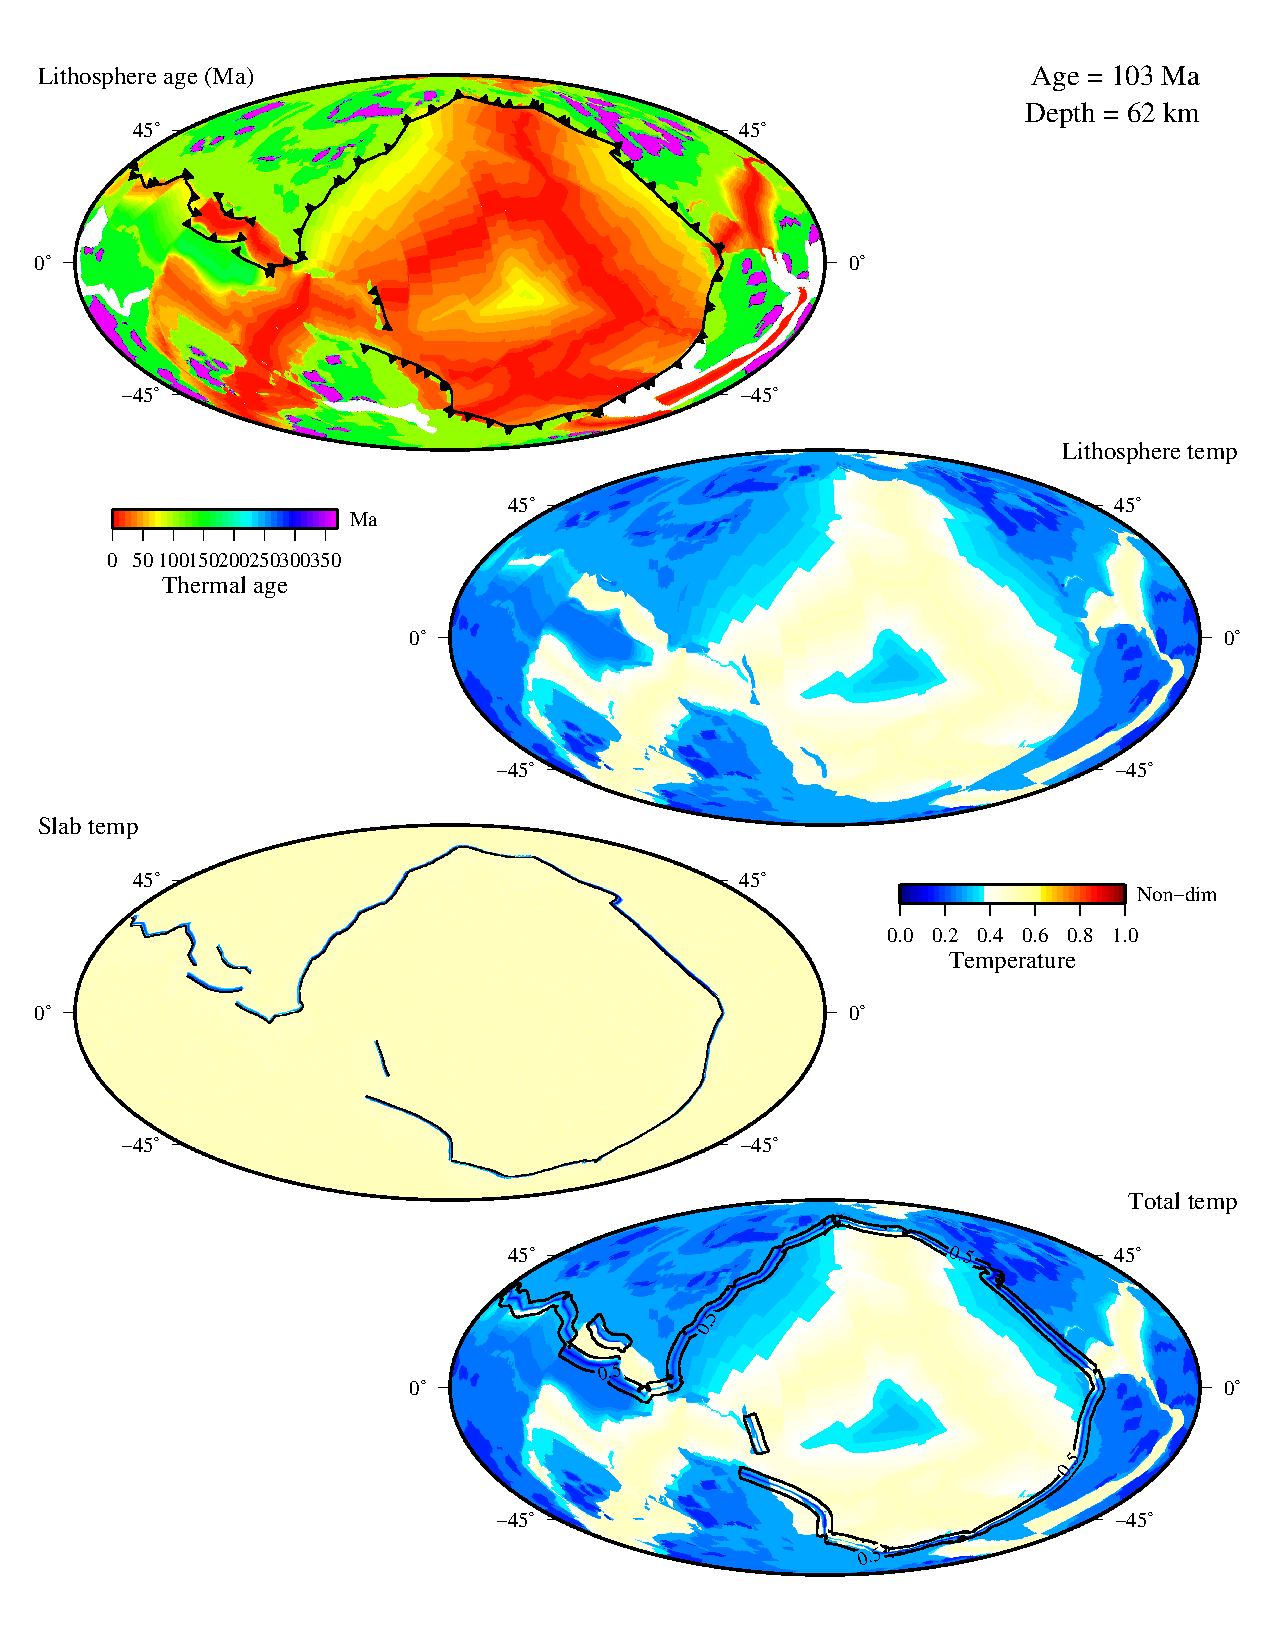
\includegraphics[width=0.6\textwidth]{figs/temp_62km_103Ma}
\end{figure}

\begin{figure}[htb]
\caption{\textit{(Previous page.)} Example of \texttt{temp.DEPTHkm.AGEMa.ps} from the global case. The top panel show lithospheric ages (no-assimilation areas are in white) and subduction zones. The second panel shows the lithosphere temperature to be mapped to CitcomS. The third panel shows subduction zones as black line and the temperature structure to be mapped to CitcomS. The bottom panel shows the merged lithosphere and slab temperature to be assimilated in CitcomS, as well as the contours of the slab stencil.}
\label{fig:stencileg}
\end{figure}

\subsection{Internal velocity assimilation files}
Internal velocity files ensure that the velocity of slabs in the upper mantle is comparable to the velocity of the subducting lithosphere at the trench \citep[see][]{BGF15}.  The following paths and prefixes must be set correctly in the ``geodynamic\_framework\_defaults.conf'' file that you are using:

\begin{verbatim}
# location of gplates exported .xy velocity data (cap, and optionally, gmt)
gplates_velo_xy_dir =

# location of gplates velocity grids (after processing cap files with grid_maker.py)
gplates_velo_grid_dir =
\end{verbatim}
Create\_History.py requires that the GPlates velocity grids are named as:\\
gplates\_vx.0.[age].grd\\
gplates\_vy.0.[age].grd\\
where ``vx'' is latitudinal velocity and ``vy'' is longitudinal velocity, both with units of cm/yr.  You can create the velocity grids from the output GPlates xy velocity data using the script ``grid\_maker.py''.

In the input cfg file you must also set:
\begin{verbatim}
#============
# data output
#============

# internal velocity (slab descent)
OUTPUT_IVEL = True
\end{verbatim}

\begin{verbatim}
#========================
# data output directories
#========================
# N.B. use an absolute path for mode = parallel

ivel_dir = ./ivel/
\end{verbatim}

\begin{verbatim}
# spatial resolution of the prescribed ivel bcs
# levels = 1 ; prescribe at finest mesh
# levels = 2 ; coarsen by 2 in each dimension
# levels = 3 ; coarsen by 4 in each dimension
# for global models you'll likely need levels >= 2
# for regional models try levels = 1 and then increase
# if convergence is poor or solve time is unreasonable
levels = 2
\end{verbatim}
``ivel\_dir'' specifies the location of the output ivel files.  ``levels'' determines if the internal (slab) velocities are applied to all nodes in the CitcomS computational mesh contained within slabs or if the velocities are applied to a coarser mesh (levels$\ge$1).

\subsection{Hot blobs and silos to model plumes}
%\dbnote{Rakib to add details here}

Thermal perturbations in the form of spherical blobs or silos (cylindrical base with a hemispherical cap) can be incorporated in the models as seeds for mantle plumes. The spatial location and essential parameters needed to define these perturbations are listed below in the examples. For each category (blob/silo) multiple perturbations can be included by specifying a list of required parameters. The temperature profile within these perturbations can vary with distance, $x$, from the axis of symmetry as:

\begin{tabular}{cc}
Type & Function \\
\hline
constant            & $A$ \\
exponential         & $A exp(-\frac{x}{r})$ \\
gaussian1           & $A exp(-\frac{x^2}{r^2})$ \\
gaussian2           & $A (1 - \frac{x^2}{r^2}) exp(-\frac{x^2}{r^2})$ \\
\end{tabular}

In the functions above, $A$ and $r$ are the user-specified amplitude of a perturbation as nondimensional temperature and the radius of a perturbation, respectively.
\subparagraph{}
Additionally, a mantle adiabat can be incorporated as a linear temperature increase across the mantle as shown below.

\begin{verbatim}
# thermal blobs
BUILD_BLOB = False ; thermal blobs
blob_center_lon = 50, 130 ; degrees
blob_center_lat = 45, 45 ; degrees colat
blob_center_depth = 2867, 2867 ; km
blob_radius = 200, 400 ; km
blob_birth_age = 230, 220 ; Ma
blob_dT = 0.1, 0.1 ; non-dimensional temperature anomaly
blob_profile = constant, constant ; valid profiles (constant,exponential,gaussian1,gaussian2)

# thermal silos
BUILD_SILO = False ; thermal silos
silo_base_center_lon = 50, 130 ; degrees
silo_base_center_lat = 90, 90 ; degrees colat
silo_base_center_depth = 2867, 2867 ; km
silo_radius = 200, 400 ; km
silo_cylinder_height= 500, 500 ; km
silo_birth_age = 230, 220 ; Ma
silo_dT = 0.1, 0.1 ; non-dimensional temperature anomaly
silo_profile = constant, constant ; valid profiles (constant,exponential,gaussian1,gaussian2)

# with ADIABAT, temperatures are re-normalized [0,1] at output
# only for extended-Boussinesq or compressible models
BUILD_ADIABAT = False ; linear temp increase across mantle
adiabat_temp_drop = 0.3 ; non-dim w.r.t. super-adiabatic
\end{verbatim}

\subsection{Assimilation of a thermo-chemical continental lithosphere}

Compositionally distinct continents can be incorporated in the models, which is particularly relevant to investigate changes in isostatic topography in models based on tectonic reconstructions with deforming plates.  We consider the first-order thermal (cold lithosphere) and chemical (light, buoyant lithosphere) characteristics that distinguish continental lithosphere from the convecting mantle.  In addition, we consider different continental types, in this example based on the simplified tectonothermal age of the continents (Archean, Proterozoic and Phanerozoic).  Continental types may be defined differently depending on the purpose of the models.

\subsubsection{Exporting xy data from GPlates (continent specific)}
\label{sssect:input_export_cont}

\paragraph{Exporting continental types}

The reconstructed continental types, defined as polygons, must be exported through time.  In the current workflow we use the series of files available in:\\
\gplatesmodel StaticGeometries/ContinentalStencils/

\begin{verbatim}
[ContinentalStencils]$ ls -1
Archean_fixed_poles_extended.gpml
Blocks_crossing_Poles.rot
Phanerozoic_fixed_poles.gpml
Proterozoic_fixed_poles_extended.gpml 
\end{verbatim}

Load these files in GPlates along with the global rotation file ( \gplatesmodelrot ); connect the file Blocks\_crossing\_Poles.rot to the global rotation file (Section~\ref{sect:GPlates}).  These files can then be exported from GPlates as follows:

Select the menu item \gp{Reconstruction $\rightarrow$ Export ...}.

In the Export Menu Dialog check the \gp{Export Time Sequence of Snapshots} button, 
and adjust the Animate time from 103 Ma to 0 Ma.  Keep the default increment of 1 Ma.

Now we will add entries for Reconstructed Geometries to the Export Data list.
Select \gp{Add Export Type} and set the export options in boxes 1 to 4.

\begin{itemize}
\item Box 1: choose Data Type to Export, select \gp{Reconstructed Geometries}.
\item Box 2: choose Output File, Format Select \gp{GMT (*.xy)}.
\item Box 3: configure Export Options, untick \gp{Export to a single file}.
\item Box 4: specify Output Filenames, keep the default file name Template: \gp{reconstructed\_\%0.2fMa}.
\item Click \gp{OK}.
\end{itemize}

You will return to the Main Export Dialog Box.

\begin{itemize}
\item Next to Target Directory, use the \gp{...} button to open a file dialog.
\item Navigate to your working copy of ``Continental\_types\_TEST''.
\end{itemize}

You will return to the Main Export Dialog Box.

\begin{itemize}
\item Click \gp{Begin Animation} to export all of the .xy data files.
\end{itemize}

A series of xy files will be created under three directories in our case.

\begin{verbatim}
[Continental_types_TEST]$ ls -1
Archean_fixed_poles_extended
Phanerozoic_fixed_poles
Proterozoic_fixed_poles_extended
\end{verbatim}

The exported continental types are used to make global age grids with ages for the oceanic and continental lithospheres.
Each continental type is assigned a negative integer to distinguish continents from oceans.
These integers will later be mapped to a thermal lithospheric thickness.
The age grids with oceans and continents are typically called agegrid\_final\_with\_continents\_220.grd where 220 is the age in million years.

\paragraph{Exporting ``no-assimilation" stencils}

The age (thickness) of the thermal lithosphere should be assimilated in rigid areas, but not in deforming areas so that the thermal structure can evolve much more naturally through advection--diffusion and the over-riding deforming plate.
Therefore, the shape of the deforming plate networks must be exported from GPlates to be made into no assimilation ``stencils''.
This is straightforward when deformation continues  onto the present day where the shape of the deforming areas can be exported directly from the deforming networks:

Select the menu item \gp{Reconstruction $\rightarrow$ Export ...}.

In the Export Menu Dialog check the \gp{Export Time Sequence of Snapshots} button, 
and adjust the Animate time from 103 Ma to 0 Ma.  Keep the default increment of 1 Ma.

Now we will add entries for Resolved Topologies to the Export Data list.
Select \gp{Add Export Type} and set the export options in boxes 1 to 4.

\begin{itemize}
\item Box 1: choose Data Type to Export, select \gp{Resolved Topologies (CitcomS specific) }.
\item Box 2: choose Output File, Format Select \gp{GMT (*.xy)}.
\item Box 3: configure Export Options, keep all the defaults set as is.
\item Box 4: specify Output Filenames, select \underline{only} \gp{Export all Network Boundaries to a single file}, keeping the default file name Template: \gp{topology\_\%P\_\%0.2fMa}.
\item Click OK.
\end{itemize}

You will return to the Main Export Dialog Box.

\begin{itemize}
\item Next to Target Directory, use the \gp{...} button to open a file dialog.
\item Create a new directory named for example ``No\_assimilation\_stencils\_2014.1''.
\end{itemize}

You will return to the Main Export Dialog Box.

\begin{itemize}
\item Click \gp{Begin Animation} to export all of the .xy data files.
\end{itemize}

When deformation ends in the past, the final geometry of the deforming network must be propagated to younger times.
Simply load the file:\\
\gplatesmodel StaticGeometries/Deforming\_networks\_static\_2014.1.gpml\\
along with the global rotation file in GPlates, and export the reconstructed geometries as GMT (*.xy) as when exporting continental types.
Merge (concatenate) the obtained .xy files with the .xy files obtained by exporting the outline of the (``dynamic") deforming networks in the proviso step. Save the resulting concatenated files as topology\_network\_polygons\_\$AGE.00Ma.xy files in a new directory, for example No\_assimilation\_stencils\_2014.1/Dynamic-Static/.
%
%\begin{itemize}
%\item Select the network at its last existing age using the select tool
%\item On the right hand side, click the middle button (\gp{Copy Geometry to Digitise Tool})
%\item Click \gp{Create Feature}
%\item Select default \gp{gpml:UnclassifiedFeature}
%\item Click \gp{Next}
%\item Specify the Plate ID and time of appearance (one million year younger than last occurrence of dynamic network) and name the feature
%\item Click \gp{Next}
%\item Click \gp{Next}
%\item Select \gp{Create a new feature collection}
%\item Click \gp{Create and Save} 
%\item Click \gp{Save as}
%\end{itemize}
%Name the Feature collection (for example No\_assimilation\_stencils\_static.gpml)
%
%Re-iterate the operation for each network; only the last step is different: add the subsequent networks to the existing Feature Collection No\_assimilation\_stencils\_static.gpml

\subsubsection{Age files for lithosphere assimilation with continents}
\label{sssect:input_age_cont}

The procedure to create age files using make\_history\_for\_age.py for lithosphere assimilation is similar to that described in Section~\ref{ssect:input_age} with a few additions.

Ensure that the following paths and prefixes are set correctly in the ``geodynamic\_framework\_defaults.conf'' file that you are using:

\begin{verbatim}
# path to age grids with (continental) mask
age_grid_mask_dir =
age_grid_mask_prefix = agegrid_final_mask_

# if using continents, path to age grids with continental ages
age_grid_cont_dir =
age_grid_cont_prefix = agegrid_final_with_continents_

# location of no assimilation stencils (after merging dynamic deforming polygons from GPlates
# and static, "ghost" polygons)
no_ass_dir =
\end{verbatim}

In the configuration file for Create\_history.py (your copy of config.cfg), set

\begin{verbatim}
CONTINENTAL_TYPES = True
\end{verbatim}

Continental types identified by negative integers are then each assigned an age in order to obtain the desired lithospheric thickness of the thermal lithosphere from the half-space cooling model following $y_L = 2.32\,\sqrt{\kappa t}$, where $y_L$ is the thickness of the lithosphere, $\kappa$ the thermal diffusivity and $t$ the age of the lithosphere.
Note that the ages used in the following do not have a geological meaning: we are simply using the lithospheric assimilation routines to obtain the desired thickness of the thermal lithosphere.

In the example below
\begin{verbatim}
stencil_values=-4,-3,-2,-1
stencil_ages=104,103,153,369
\end{verbatim}

Archean continents (-1) are 250 km thick, Proterozoic (-2) continents are 160 km thick and all other continents are 130 km thick.

To obtain fully dynamic deforming zones, set 

\begin{verbatim}
NO_ASSIM = True
no_ass_age = -1000
no_ass_padding = 100
\end{verbatim}

The value no\_ass\_age should be smaller than -999 (-1000 by default) and the value no\_ass\_padding (km) creates a no-assimilation buffer zone intended for narrow deforming areas such as passive margins.

\subsubsection{Buoyant continents using numerical tracers}
\label{sssec:make_tracers}
In this step, a global tracer file is mapped from the (GMT) age grid at the age of the initial condition to CitcomS-format input data files (ascii).

In the configuration file for Create\_history.py (your copy of config.cfg), set

\begin{verbatim}
# tracer initial condition
OUTPUT_TRAC_IC = True
\end{verbatim}

The (very large) tracer file model\_name.tracer.\$\{AGE\}Ma will be written in the folder:

\begin{verbatim}
#========================
# data output directories
#========================
# N.B. use an absolute path for mode = parallel

trac_dir = ./trac/
\end{verbatim}

The number of tracers per element is given by: 

\begin{verbatim}
#=========================
# tracer initial condition
#=========================
# this is approximate, because tracers are uniformly distributed
tracers_per_element = 30
\end{verbatim}

The tracers are then mapped to CitcomS from the (GMT) age grids with continents using the stencil\_values defined in the previous step (section~\ref{sssect:input_age_cont}).

In this example, we have five geological ``terrane'' types: oceanic, Phanerozoic, Proterozoic, Archean.  For simplicity, we have taken the thickness of the chemical lithosphere (defined below by depth\_stencil\_value\_ in km) equal to that of the thermal lithosphere (defined in the previous step by stencil\_ages in Ma - stencil ages are converted to depths according to the half-space cooling model). 

\begin{verbatim}
# Build tracer field with continents using 'stencil_values'
# tracer flavors and depths

# for positive thermal ages (i.e., oceanic)
# note: must be '0' suffix
flavor_stencil_value_0 = 0
depth_stencil_value_0 = 410

# for stencil value -1
flavor_stencil_value_1 = 1,2
depth_stencil_value_1 = 40,250

# for stencil value -2
flavor_stencil_value_2 = 1,3
depth_stencil_value_2 = 40,160

# for stencil value -3
flavor_stencil_value_3 = 1,4
depth_stencil_value_3 = 40,130

# for stencil value -4
flavor_stencil_value_4 = 1,4
depth_stencil_value_4 = 40,130

# etc. for more stencil values, e.g.,
# flavor_stencil_value_5 = 0 
# depth_stencil_value_5 = 410
\end{verbatim}

In addition, it is desirable to remove continental tracers next to subduction zones for numerical reasons (specifically to limit the entrainment of buoyant tracers to depth). This can be done using the following parameter:

\begin{verbatim}
# set region around slabs to ambient flavor (0)
SLAB_STENCIL = True
# stencil width: 300 km is consistent with the default width of the thermal stencil
# wide stencils limit crustal thickening along convergent margins
# narrow stencils avoid a gap along convergent margins but may result in significant
# crustal thickening and unrealistic elevations along convergent margins
slab_stencil_width = 300 ; km - suggested range: 100-300 km
\end{verbatim}

The postscript files produced by the script will show the continental types used to create tracers (Fig.~\ref{fig:cont2ps}).

\begin{figure}[htb]
\centering
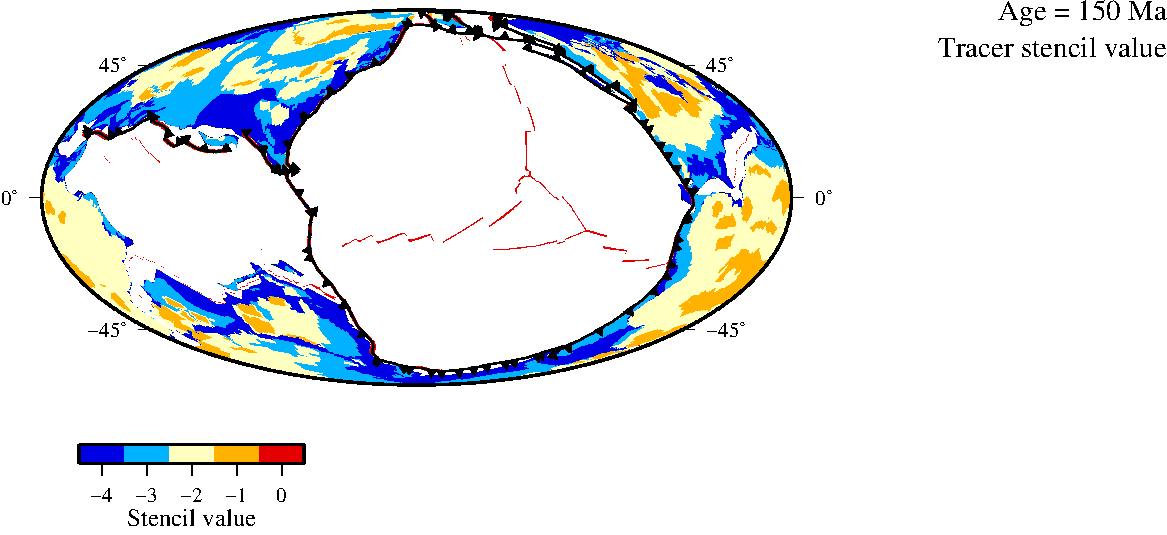
\includegraphics[width=0.6\textwidth]{figs/tracer_150Ma}
\caption{Example of mapped continental types for a global case starting at 150~Ma \texttt{(tracer.AGEMa.ps)}. }
\label{fig:cont2ps}
\end{figure}

A deep layer can also be added to model the evolution of chemical piles by using:

\begin{verbatim}
# uniform dense layer at base of mantle
DEEP_LAYER_TRACERS = True
deep_layer_thickness = 300 ; km - 113 km gives 2 per cent of Earth's volume.
# flavor should not be 0 (0 is always ambient flavor)
deep_layer_flavor = 5
\end{verbatim}

You will want to ensure that deep\_layer\_flavor is different to the previously defined flavors.

Finally, for numerical efficiency, the option is given to remove tracers for a set depth range:

\begin{verbatim}
# eliminate tracers between these bounds
# this saves memory when using the hybrid method to compute composition
NO_TRACER_REGION = True
no_tracer_min_depth = 410 ; km
no_tracer_max_depth = 2604 ; km
\end{verbatim}

If NO\_TRACER\_REGION is ``True" then ``hybrid\_method'' must also be set to ``1" in the input file of the CitcomS run:

\begin{verbatim}
[CitcomS.solver.tracer]
tracer = on
hybrid_method = 1
\end{verbatim}

The ``hybrid method'' is similar to the ``ratio method'' \citep[see][]{TK03}  to compute composition, except that composition is assumed to be ``ambient" (0) if no tracers are present in an element (see Section~\ref{ss:assim_param} for more details).  For certain types of problems, the hybrid method is an advantageous approach because:
\begin{itemize}
\item Fewer tracers are required, which saves time in the composition advection routine.
\item For most parts of the domain, the preferred statistical characteristics of the ratio method are retained (effectively, fewer tracers are required in these regions versus the absolute method, see \cite{TK03}).
\end{itemize}

Upon running, the script outputs the PS file surface\_types.ps that allows the user to check the correct definition of the continental types in map view (Figure 7).

To scale continental elevations, the chemical buoyancy of the different tracers must then be adjusted by iteratively running the initial condition for the final CitcomS run.

\subsection{Synthetic (regional) models}
We develop synthetic regional models in \cite{BGF15} to demonstrate that the slab buoyancy flux is comparable to the flux of the lithosphere at the trench.  See Case K, 1--10, in the paper.  These models are developed using entirely synthetic data that is constructed using the following parameters in the input cfg:

\begin{verbatim}
#==============================
# synthetic regional model only
#==============================
SYNTHETIC = False ; master switch for synthetic regional models
OUTPUT_BVEL = True ; output velocity boundary conditions
bvel_dir = ./bvel ; bvel
fi_trench = 0.8 ; radians
TRENCH_CURVING = False
curving_trench_lat = 0.0 ; degrees
subduction_zone_age = 100 ; Ma
plate_velocity = 5 ; cm/yr
plate_velocity_theta = -1 ; direction of velocity (non-dim)
plate_velocity_phi = 1 ; direction of velocity (non-dim)
velocity_smooth = 200 ; bvel smoothing (Gaussian filter)
no_of_edge_nodes_to_zero = 3 ; no of edge nodes to smooth across (x and y)
overriding_age = 50 ; Ma
rollback_start_age = 100 ; Ma
rollback_cm_yr = 0 ; cm/yr (direction is always -phi)
\end{verbatim}

\subsection{Regional models}
The difference in the assimilation work flow between regional and global models mainly rest with the generation of surface velocity data. To export surface velocity data files in regional models, you need to follow these several steps:

\paragraph{Generate CitcomS coor file}
You can use \textit{Make\_citcoms\_coord\_file.py} to generate an uneven (or even if you like) CitcomS mesh file. e.g. 
\begin{verbatim}
Make_citcoms_coord_file.py -v -f Coord.cfg
\end{verbatim}
Where Coord.cfg is the controling file you give. Here is an example of the cfg file:
\begin{verbatim}
name_prefix = Nz65
verbose = True

nproc_surf = 1
nodex = 129
nodey = 129
nodez = 65

degrees_or_radians=degrees
#degrees_or_radians=radians
# Establish the regional domain
#   The map coordinates can either be given as degrees in geographical
#   coordinates (lat, lon) or in radians (colat., long)
lat_min = -35.0
lat_max = 45.0
lon_min = 75.0
lon_max = 155.0
#theta_min=0.8727
#theta_max=2.0944
#fi_min=1.3963
#fi_max=2.6180

radius_outer = 1.0
radius_inner = 0.55

# Give the refinement details
# if refinement_ratio_theta, refinement_ratio_fi NOT given
# then there will be no refinement in that direction
#
#If degrees_or_radians is set to degrees, above, then these
# are interpreted as degrees
#refinement_ratio_theta = 4.0
#refinement_coor_theta = 30.0
#refinement_width_theta = 5.0
#refinement_ratio_fi = 3.0
#refinement_coor_fi = 275.0
#refinement_width_fi = 10.0

refinement_lower_width=0.005
refinement_lower_ratio=3
refinement_upper_width=0.005
refinement_upper_ratio=6.0
\end{verbatim}

\textit{Make\_citcoms\_coord\_file.py} can generate this sample config file with the '-e' command like this:

\begin{verbatim}
Make_citcoms_coord_file.py -e > Coord.cfg
\end{verbatim}


\paragraph{Generate gpml mesh file based on the regional CitcomS coor file}
To make GPlates able to export regional velocity data, you need to create a gpml format file based on the CitcomS coor file. Run \textit{convert\_meshes\_citcoms\_to\_gpml.py} under the directory same as the CitcomS coor files in the following form to generate a gpml file:
\begin{verbatim}
convert_meshes_citcoms_to_gpml.py format_name in_file out_file
\end{verbatim}
Where \textit{format\_name} must be set as one of:  \[\textbf{citcoms\_regional, citcoms\_global or citcoms\_regional\_cap}\]
For regional model, \textit{in\_file} is name of the citcoms coor file and \textit{out\_file} is the prefix of output gpml format file. You must set \textit{out\_file} as \emph{0.mesh.0} for regional model to make it readable by GPlates. e.g.
\begin{verbatim}
convert_meshes_citcoms_to_gpml.py citcoms_regional Nz65.coor.regional.dat 0.mesh.0
\end{verbatim}

\paragraph{Output velocity file by gplates}
Now we will use gplates to export the surface velocity data for CitcomS calculation.
First, select the menu item \gp{File $\rightarrow$ Open Feature Collection} to read in the gpml mesh file (Note that GPlates will export regional CitcomS velocity data only if the input .gpml file has exactly the name \emph{0.mesh.0.gpml}).

Second, just as you did in Section 2.5 for the global model, select the menu item \gp{Recinstruction $\rightarrow$ Export $\rightarrow$ Velocities $\rightarrow$ CitcomS global} to export the velocity data. Similar as the global model, the output velocity has the form as:
\begin{verbatim}
bvel${Age}.0
bvel${Age}.0.xy
\end{verbatim}
Finally, different from the global model, this format of data can not be read by CitcomS directly. Regional CitcomS read in velocity data with the format as:
\begin{verbatim}
bvel${Age}
\end{verbatim}
So you need to perform some simple transformation to the velocity file names. Here is one example shell script:
\begin{verbatim}
#!/bin/sh
cp bvel50.0 bvel51.0
cp bvel50.0.xy bvel51.0.xy
for i in `seq 0 1 52`
do
mv ./bvel${i}.0  ./bvel${i}
mv ./bvel${i}.0.xy  ./bvel${i}.xy
done
\end{verbatim}
You need to change the ages in the script based on your own cases.

\section{Compiling and running CitcomS for data assimilation}
\subsection{Obtain the base code}
Parts of the following instructions are taken directly from the CitcomS manual and you should read sections 2.10--2.13.3 of the current (v3.2.0) user manual available from the CIG website \url{http://www.geodynamics.org/cig/software/CitcomS}.

In addition to the usual system requirements, you will need a handful of additional development tools installed in order to work with the source from the CIG software repository.  First, you must have a Subversion client installed.  To check, type svn; it should return a usage message.

\tm{svn} \\
\tmo{Type `svn help' for usage.}

For more information on Subversion, visit the Subversion website \url{http://subversion.apache.org}.
Second, you must have the GNU tools Autoconf, Automake, and Libtool installed.  To check, enter the following commands:
\begin{itemize}
\item \tm{autoconf --version}
\item \tm{automake --version}
\item \tm{libtoolize --version}
\end{itemize}
To check out the latest version of CitcomS, use the svn checkout command:

\tm{svn checkout https://geodynamics.org/svn/cig/mc/3D/CitcomS/trunk CitcomS-assim}

This will create the local directory `CitcomS-assim' (if it doesn't already exist) and fill it with the latest CitcomS source from the CIG software repository.  The CitcomS directory thus created is called a working copy.  Use the update command to obtain version 16400:

\tm{cd CitcomS-assim}\\
\tm{svn up -r16400}

Unfortunately there is a bug in version 16400 that produces incorrect mechanical boundary conditions.  To solve this problem we `back-out' the following files in the `lib' directory to version 16022 by issuing the following commands:

\tm{cd lib}\\
\tm{svn up -r16022 Ggrd\_handling.c Full\_boundary\_conditions.c BC\_util.c Topo\_gravity.c \\Regional\_boundary\_conditions.c }

At this stage you now have an operational `base code'.  However, note that ggrd functionality is likely broken in this base code because it was still being developed at this time (by a different user).  However, we do not use ggrd functionality for data assimilation.

\subsection{Patch the base code for data assimilation}

\textbf{Important:} The data assimilation patches were specifically written for the Pyre version of CitcomS and therefore are not expected to work with the C-version without further development.

There is another svn that contains the modified files that are necessary to patch the base code to provide data assimilation functionality.  Use the svn checkout command (note that you will need checkout privileges):

\tm{svn checkout https://svn.gps.caltech.edu/repos/CitcomS CitcomS-patch}

Manually copy-and-replace the modified files from CitcomS-patch/CitcomS into your working copy of CitcomS-assim.   Ensure that you copy the modified files into exactly the same directory structure as they appear in CitcomS-patch/CitcomS.

Below is a complete list of files that should be copied:
\begin{itemize}
\item CitcomS/Components/BC.py
\item CitcomS/Components/Param.py
\item CitcomS/Components/Tracer.py
\item CitcomS/Solver/Solver.py
\item lib/Advection\_diffusion.c
\item lib/BC\_util.c
\item lib/Composition\_related.c
\item lib/composition\_related.h
\item lib/Convection.c
\item lib/Element\_calculations.c
\item lib/Full\_boundary\_conditions.c
\item lib/Full\_lith\_age\_read\_files.c
\item lib/Full\_read\_input\_from\_files.c 
\item lib/Full\_solver.c
\item lib/global\_defs.h
\item lib/Instructions.c
\item lib/Lith\_age.c
\item lib/Output.c
\item lib/Problem\_related.c
\item lib/Regional\_boundary\_conditions.c
\item lib/Regional\_lith\_age\_read\_files.c
\item lib/Regional\_read\_input\_from\_files.c
\item lib/Regional\_solver.c
\item lib/solver.h
\item lib/Stokes\_flow\_Incomp.c
\item lib/tracer\_defs.h
\item lib/Tracer\_setup.c
\item lib/Viscosity\_structures.c
\item module/bindings.c
\item module/misc.c
\item module/misc.h
\item module/setProperties.c
\item m4/cit\_python.m4 \footnote{m4/cit\_python.m4 was changed around August 2011 by the pylith team to fix a bug in Merlin.  However, the change disabled the automatic download of Pythia that we require for CitcomS.  Therefore it may be necessary to copy-and-replace this file to prevent the code from exiting with the following error when you run \tm{./configure}:\\
\tmo{configure: Generating Python egg info\\checking for egg-related flags... failed\\configure: error: cannot scan Python eggs for flags}}
\end{itemize}

In addition, the ``deps'' directory includes merlin and pythia versions that are currently used for the Citerra installation.  If \tm{./configure} is unable to download the egg files, try copying and pasting the ``deps'' directory into your CitcomS-assim directory.

\subsection{Load modules (Citerra specific)}
On Citerra you need to load certain modules in the terminal window each time you want to compile your CitcomS code.  You do not need to load the modules to submit jobs to the queue manager; they are only required when compiling the code.  I use the intel compiler and mpi implementation:

\tm{module load intel/intel-12 intel/impi}

You can check the modules are loaded correctly:

\tm{module list}

At present, the default Python version on Citerra is 2.4.3, which is suitable for compiling CitcomS with Pyre.  According to the CitcomS manual (v3.2.0), ``Pyre in CitcomS does not work with Python 2.7 or higher'', although I think incompatibilities have also been reported with some versions of Python 2.6.
\subsection{Compile CitcomS}
Navigate to the top level of your CitcomS code (CitcomS-assim) and run the following commands:
\begin{itemize}
\item \tm{make distclean} \footnote{Remove all files made by previous builds.}
\item \tm{autoreconf -i --force}
% \item \tm{rm -r deps}
\item \tm{./configure}
\item \tm{make}
\end{itemize}

Note that the assimilation framework requires CitcomS be installed with Pyre (see CitcomS manual).
\subsection{Change the Scheduler}
Most users have a configuration file that contains the scheduler information, although that you can also include the scheduler commands in a regular CitcomS .cfg file.

The following steps assume that \verb#$HOME/.pyre/CitcomS/CitcomS.cfg# exists.  If it doesn't, create it.
%\item Backup original configuration file, which should contain the LSF scheduler.\begin{verbatim}
%cp $HOME/.pyre/CitcomS/CitcomS.cfg $HOME/.pyre/CitcomS/CitcomS_lsf.cfg
%\end{verbatim}
Ensure your \verb#$HOME/.pyre/CitcomS/CitcomS.cfg# looks exactly like this:

\begin{verbatim}

[CitcomS]
scheduler = pbs

[CitcomS.launcher]
command = /opt/intel/impi/4.0.3.008/bin/mpirun -np ${nodes} -machinefile ${PBS_NODEFILE}

[CitcomS.job]
queue = default
\end{verbatim}
There is also a \verb#[CitcomS.pbs]# group, but you shouldn't need to use this unless you wish to specify advanced options with your job submission.

You should now be able to submit and run jobs.
\subsection{Monitor jobs (Citerra specific)}
Citerra uses the Maui scheduler and Torque resource manager, and the commands are a little different from LSF.
\begin{itemize}
\item To view jobs in the queue: \tm{showq} or \tm{qstat}
\item To diagnose a job: \tm{checkjob}
\item To delete a job: \tm{qdel}
\end{itemize}
\subsection{Path (bash specific)}
If you are only working with one installation of CitcomS-assim, or have a preferred default, then you can add the following lines to your \$HOME/.bash\_profile so you can call the binary by simply typing \tm{CitcomS} rather than the full path name.  Change the CitcomS\_DIR variable to the path of your CitcomS-assim directory.  For example, your modified \$HOME/.bash\_profile will contain entries similar to these:
\begin{verbatim}
CitcomS_DIR=cig/CitcomS
export PATH=$HOME/$CitcomS_DIR/bin:$PATH
\end{verbatim}
Finally, remember to apply your changes by re-sourcing:\\
\tm{source \$HOME/.bash\_profile}

\subsection{Assimilation parameters}
\label{ss:assim_param}
CitcomS with assimilation includes several new parameters that can be included in the input model *.cfg file:
\begin{itemize}
\item \verb#[CitcomS.solver.ic] mantle_temp#\\ set to the exact ``temperature\_mantle'' used in your Create\_History.py input cfg file.  This is critical for lithosphere assimilation to be implemented correctly!
\item \verb#[CitcomS.solver.param] slab_assim#\\ set thermal slab assimilation on (1) or off (0)
\item \verb#[CitcomS.solver.param] slab_assim_file#\\ prefix for thermal slab assimilation files
\item \verb#[CitcomS.solver.param] lith_age_depth_function#\\ set on (1) or off (0, default).  Lithosphere assimilation depth is a function of the lithosphere age according to the following equation (see Eq. 4--126 of Turcotte and Schubert):
\begin{equation}
\label{eqn:lith_assim_depth}
\textrm{Lithosphere assimilation depth} =  \textrm{max}(\textrm{lith\_age\_depth} \times 2.32 \times (\sqrt{\textrm{Age} \times \kappa}) / R_0, \textrm{lith\_age\_min})
\end{equation}
Note that:
\begin{enumerate}
\item \verb#[CitcomS.solver.param] lith_age_depth# is redefined as a prefactor ($\approx 1-2$).  By default, with \verb#lith_age_depth_function# turned off, \verb#lith_age_depth# is the actual assimilation depth ($\approx 0.01-0.05$).
\item \verb#[CitcomS.solver.param] lith_age_min# is used to define a minimum lithosphere assimilation depth.  Using Eqn.~\ref{eqn:lith_assim_depth}, \verb#lith_age_min# = 23.9 (Ma) gives a minimum lithosphere assimilation depth = 0.01.
\item Besides the above, \verb#[CitcomS.solver.param] lith_age_min# is otherwise unused in CitcomS for data assimilation.
\end{enumerate}
\item \verb#[CitcomS.solver.param] file_internal_vbcs#\\ set internal velocity boundary conditions on (1) or off (0)
\item \verb#[CitcomS.solver.param] vel_internal_file#\\ prefix for internal velocity boundary condition files
\item \verb#[CitcomS.solver.output] output_optional#\\ can additionally include \verb#divv, comp_sph, temp_sph, sten_temp, sten_velo, tracer_dens# for the divergence of velocity\footnote{The convergence criteria for CitcomS is specified as the absolute value of the divergence of the velocity normalized by the magnitude of the velocity.  You will need to post-process the divv output to achieve the same quantity because divv is only the divergence of the velocity.}, spherical harmonic expansion of composition\footnote{Not extensively tested.}, spherical harmonic expansion of temperature, thermal stencil, velocity stencil, and tracer density, respectively.  The velocity stencil is 1 for nodes that are turned on and 0 for nodes that are turned off.
\item \verb#[CitcomS.solver.tracer] hybrid_method#\\ this switch activates what we call the ``hybrid method'' for determining composition.  Essentially the method follows the same algorithm as for the ``ratio method'', only if an element is devoid of tracers the composition of that element is automatically assigned to ambient composition (zero).  This method is useful for these reasons: (1) the code does not crash when too few tracers are in an element.  (2) input tracer files can be much smaller because the whole domain does not need to be filled with tracers.  (3) Advection of the tracers takes less time (because there are less of them).
\item \verb#[CitcomS.solver.param] exclude_buoy_above_znode#\\ set on (1) or off (0).  Off by default.
\item \verb#[CitcomS.solver.param] exclude_buoy_znode#\\ include all buoyancy sources (temperature, composition, phase) at and below this specified znode (must be an integer) in the RHS of the Stokes solver.  Buoyancy at znodes greater than the specified znode is explicitly set equal to zero at each time step.  The CMB ($r=0.55$ by default) is at znode=1 and the znodes (always integers) increase towards the surface.  Useful for the calculation of dynamic topography.
\end{itemize}



\section{Restarting CitcomS for dynamic topography and total topography (restart\_citcoms.py)}
The script ``restart\_citcoms.py'' is used to build upon a master CitcomS run and create a series of input files for secondary restart runs.  These restart runs are used to generate dynamic and total topograhy data.  As with most tools in the geodynamic framework this script uses an input configuration file (.cfg), and the script will produce an example .cfg file by using the "-e" option:

\tm{restart\_citcoms.py -e}

This .cfg file is self-documented, and the intent is that you need to change specific parameters to match the master run.
You must change the values for master run's original cfg file and original pid file ("master\_run\_cfg" and "master\_run\_pid")
You must select which ages you want to restart from ("restart\_ages"),
and select which type of restart you are performing ("restart\_type").

The script ``restart\_citcoms.py'' sets up a sub directory for the restart runs, and makes multiple modified copies of the master run's original .cfg file, one copy for each of the ages.
It adjusts various parameters in these secondary .cfg files to refect that these are restart runs, not regular runs.

The default parameters and values that are adjusted are contained in the "dynamic\_topography\_restart\_params" variable of the Core\_Citcoms.py module.
You may include other specific input .cfg parameters you wish to change for the restarts.  See the bottom section of the example ``restart\_citcoms.py'' configuration file.

Additonal information is contained in the ``restart\_citcoms.py'' example config file.

\subsection{Dynamic topography}

A Dynamic topography restart also requires these two parameters be set ("lithosphere\_depth\_DT" and "lithosphere\_temperature\_DT") in the ``restart\_citcoms.py'' configuration file.

\subsection{Total topography}

A Total topogrphy restart does not requrire any additional settings in the ``restart\_citcoms.py'' configuration file.



\section{Grid Making (grid\_maker.py)}

We have developed a script ``grid\_maker.py'' that directly processes CitcomS data 
and produces GMT4 grids for select time steps (or ages, or run times).  
It can process both volume data (e.g., temperature, composition, etc.) and surface data (e.g., surface topography, heat flux, etc.).  
Furthermore, the script can automatically dimensionalize the non-dimensional output from CitcomS to produce datasets 
that can be compared directly with observations (e.g., surface heat flux).  
The dimensionalizations are computed using the values in the CitcomS pid file to ensure that the post-processed data 
is entirely consistent with the model run.  For completeness we list the dimensionalizations that the script uses below.

Like most scripts in the geodynamic framework ``grid\_maker.py'' will give a help message if run without any arguments. 
``grid\_maker.py'' uses an input configuration file (.cfg), and the script will produce an example .cfg file by using the "-e" option:

\tm{grid\_maker.py -e}

The example file is self-documenting and contains descriptions of the various parameters.  
There are four main sections to ``grid\_maker.py'''s input:

\begin{itemize}
\item 1. Model coordinate information: "pid\_file" and "coord\_dir"
\item 2. Time values to grid: ``time\_spec"
\item 3. Levels to grid: "level\_spec"
\item 4. Fields to grid
\end{itemize}

Each section has example settings for both CitcomS model data and for GPlates velocity data.  
For any single use of ``grid\_maker.py'' only one data type (CitcomS or GPlates) is used.

In Section 1 you will set the model coordinate information common to both source types using "pid\_file" and "coord\_dir".

Please NOTE: you may have to edit the "datadir" entry in your pid\_file to reflect the proper paths.
For example the Citcom model may have been run on a different machine than the machine used for post-processing.
Often the datadir entry can be set to a relative path: "datadir=./data/\%RANK"

In Section 2 you will choose which output times to grid using "time\_spec".
A variety of forms for selecting the times are valid (single time, comma separated list, start/stop/step) and you will chose one form.  
Because of the nature of the computation model the output time in Millions of Years Ago may not match your request exactly.  
We have algorithms to choose the closest available output timestep and convert that value to Ma.  
For example you may set "time\_spec = 0Ma/30Ma/10Ma" but the closest output times are actually: 7Ma, 20Ma, 29Ma.

In Section 3 you will choose which levels to grid using "level\_spec".
A variety of forms for selecting the times are valid (single time, comma separated list, start/stop/step) and you will chose one form.
For Volume data fields the level\_spec may be values from 0 to nodez-1.
For Surface (surf) data fields the level\_spec must be set to only nodez-1.
For Botttom (botm) data fields the level\_spec must be set to only 0.
Future versions of ``grid\_maker.py'' may automaticall override these settings for Surf and Bottom fields, but for now you must match the correct level(s) to the fields.

In Section 4. you will choose which fields to grid using a set of configuration file sub blocks of this form:

\begin{verbatim}
[Grid_1]
field = temp
dimensional = True
#blockmedian_I = 0.5
#surface_I = 0.25
#Ll = ...
#Lu = ...
#T = ...
\end{verbatim}

Each block sets the gridding parameters for a single field.
The first line of the block holds a string indentifier for the field in square backets.
The next line has the requrired parameter 'field', and the cooresponding CitcomS field name. 
The CitcomS field names may be found in the official Citcoms Manual 
\url{http://www.geodynamics.org/cig/software/CitcomS/}.  
See also Core\_Citcom.py the global variable field\_to\_file\_map for more detailed field names to be used in Python scripts.
As shown above, additional optional values may be set to pass to GMT to fine tune gridding.
Additonal information is contained in the ``grid\_maker.py'' example config file.


\subsection{Heat flux}
CitcomS exports non-dimensional heat flux to *.botm.* and *.surf.* files.  Dimensionalize the heat flux for either the top or bottom surface using the following expression:
\begin{equation}
\phi = 1000 \cdot k \frac{\Delta T}{R_0} \cdot \phi^\prime
\end{equation}
where $\phi$ is dimensional heat flux (mW/m$^2$), $k$ is thermal conductivity (W/m$\cdot$K), $\Delta T$ is temperature drop ($K$), $R_0$ is Earth radius ($m$), and $\phi^\prime$ is non-dimensional heat flux (output from CitcomS).

\subsection{Dynamic and total topography}
\subsubsection{Scaling of topography}

CitcomS exports non-dimensional stress ($\sigma_{rr}$) to *.botm.* and *.surf.* files.  To dimensionalize this value we use the same scaling as equation 11 from the CitcomS manual for pressure:
\begin{equation}
P = \frac{\eta_0 \kappa}{R_0^2} P^\prime
\end{equation}
i.e.,
\begin{equation}
\sigma_{rr} = \frac{\eta_0 \kappa}{R_0^2} \sigma_{rr}^\prime
\end{equation}
where primes are non-dimensional.

Vertical stress needs to be converted to dynamic topography. We find the equivalent height for a surface to be deflected about it's equilibrium height that gives that same stress.
\begin{equation}
\sigma_{rr} = \Delta \rho g h
\end{equation}

where $h$ is the equilibrium height, $g$ is gravitational acceleration, and $\Delta \rho$ is the density difference across the top interface.  The density difference is computed using the pid file parameters ``density'' (underlying mantle $\simeq$3300 kg m$^{-3}$) and ``density\_above'' (overlying water, seawater $\simeq$1025 kg m$^{-3}$).  Therefore, $\Delta \rho$ is typically $\simeq$ 2275 kg m$^{-3}$.

Combining the two expressions for $\sigma_{rr}$ and re-arranging gives an equation for $h$:

\begin{equation}
h = \frac{1}{\Delta \rho g} \frac{\eta_0 \kappa}{R_0^2} \sigma_{rr}^\prime
\end{equation}

It is advisable to remove the mean topography since the average of dynamic topography must be zero for the whole Earth.

\subsection{Recasting Output to a Plate Frame of Reference}

The output data from CitcomS is in the fixed mantle frame of reference.  
Using a combination of tools in GPlates and options in grid\_maker.py we can re-cast the output data to the plate frame of reference.
This section outlines the steps to perform in GPlates, the grid\_maker.py options, and the settings for the Python Script 
configuration file ("geodynamic\_framework\_defaults.conf").

The first step is to identify a set of static plate polygons that coorespond 
to the same global model chosen in Section 2.2 used to create surface velocity conditions for the CitcomS run.  
This could be a complete set covering the whole globe, or some subset of plates.  
For example, this file may be used to select continental areas:

\gplatesmodel 

StaticGeometries/StaticPolygons/StaticPolygonsForPlateFrame/StaticPolygonsForPlateFrame2014.1.shp

Now we will create a set of regularly sampled points over the globe.  Open creation dialog with menu item: 

\gp{Features $\rightarrow$ Generate Velocity Domain Points $\rightarrow$ Latitude Longitude ...}

Leave the default extent (the whole globe), and change the number of 
latitudinal intervals to 180 and longitudinal intervals to 360. 
Leave the other options and file name template set to the default values.

Select the folder where you want to save the file.  
It is best to choose one of the Input directories created in Section 2.1, 
for example "sample\_case/\caserecondir/Topologies".  

This step will create a single gpml:MeshNode feature with a single multipoint geometry - 
visually you will see a set of yellow dots covering the globe (yellow because they have a default plate id set to 0).

The next step is to partition this single feature into a set of features, 
where each new feature is based upon the boundaries of the static polygons.
The partitioning will result in a group of features with single multipoint geometries: 
one-feature-per-static-polygon, with the plate ids assigned from the polygon.

Go to the menu item \gp{Features $\rightarrow$ Assign Plate IDs}.
Select the Static Polygons layer as the partitioning layer, and click Next.
Select the lat\_lon\_velocity\_domain\_180\_360.gpml layer as the layer to be partitioned, and click Next.
Other values should be left as defaults, and you may click Apply.

Now you will see several gpml:MeshNode features, each with a single multipoint geometry, and color coded acording 
to each static polygon's plate id.

If you are using static polygons that do not cover the whole Earth, (e.g. only continents) 
then any multipoints not located in any static polygon will still have a plate of if 0 (the will remain yellow). 
These points will all be in one unassigned feature, and it can be easily removed by selecting one of the points 
and clicking on the trash can in the Current Feature panel on the right side of the globe.

You may futher edit down this new feature collection to include only those particular plates or polygons you want to recast data to.
For example, if you are only interested in one plate, delete all the other features except that plate.

Be sure to save this newly partitioned feature collection - it will be highlighted red in the Manage Feature Collection dialog.
This file is now ready to be used as an input to the rest of the plate frame change workflow.

Adjust the "geodynamic\_framework\_defaults.conf" in your case data output directory to point to this file.
Set the "frame\_change\_input\_multipoint\_filename" parameter to point to the full path of this newly partitioned multipoint file.

Also confirm that the "frame\_change\_input\_rotation\_filename" entry points to the full path of the main rotation file
of the global model used in Section 2.2.

Now grid\_maker.py can automatically recast CitcomS data from the mantle frame to the plate frames with a simple option setting.  
In the global options area (above all bracket sections) set "make\_plate\_frame\_grid = True".

During the regular production of mantle frame grids, grid\_maker.py will also call an 
auxiliary script "frame\_change\_pygplates.py" with the correct options 
to transform the global data set to the plate frames as specified by 
the mutipoint features found in the "frame\_change\_input\_multipoint\_filename" file.
These additional grids will have the file name pattern "casename-fieldname-ageMa-depth-plateframe.grd".

\subsection{Creating input for 4DPlates}

4DPlates is a data viewer program developed by Simula Research Laboratory with specific tools to view geodyamic models.
To prepare your grids for use in 4DPlates you may run this command:

\begin{verbatim}
$ Core_Citcom.py -glb *.grd
\end{verbatim}

The argument is a list of grid files you wish to display in 4DPlates.  
The output will be a .glb file with data set acording to conventions and patterns found from the file names:
\begin{itemize}
\item the file name will be the same as the case name
\item the field label and id will be parsed from the file name component
\item the category will be set to "Citcoms/" with the case name appeneded 
\item the field label will be set to the reconstruction age as set in each file name component
\item the ages of appearance and disapearance will be set by the ages in the data files.
\end{itemize}

The .glb file is then used to pre-process the grid files into tiled files used by 4DPlates.
Depending on how your Windows environment is configured, you may eaither double click on the .glb file,
or use "Open With ..." and select '4DPlates\_builder'.  This data will now show up in 4DPlates in the Layers Library,
under the "Citcoms" section, with the case name.


\begin{figure}[htb]
\centering
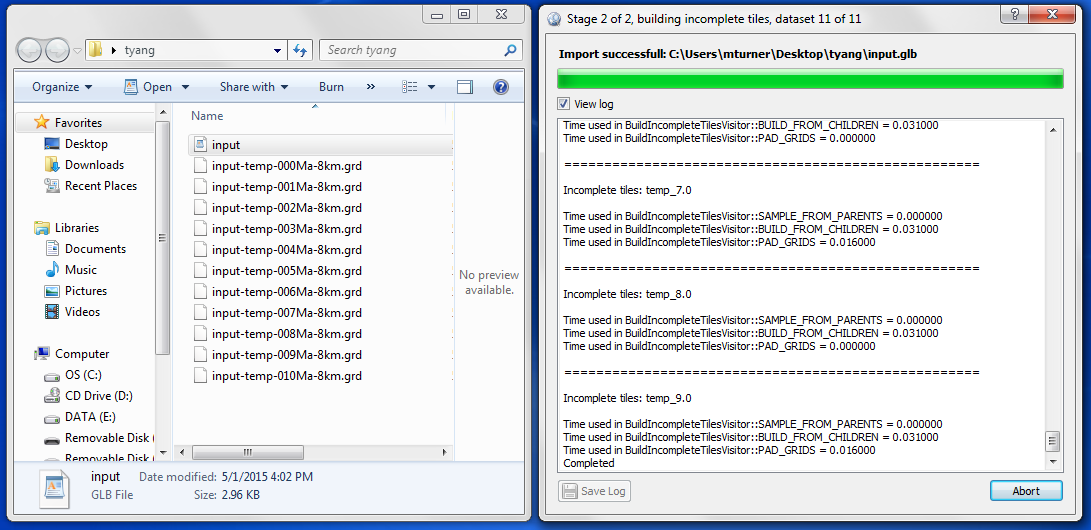
\includegraphics[width=1.0\textwidth]{figs/4DPlates_step1.png}
\caption{Step 1. Open the .glb file with '4DPlates\_builder'. }
\label{fig:cont2ps}
\end{figure}

\begin{figure}[htb]
\centering
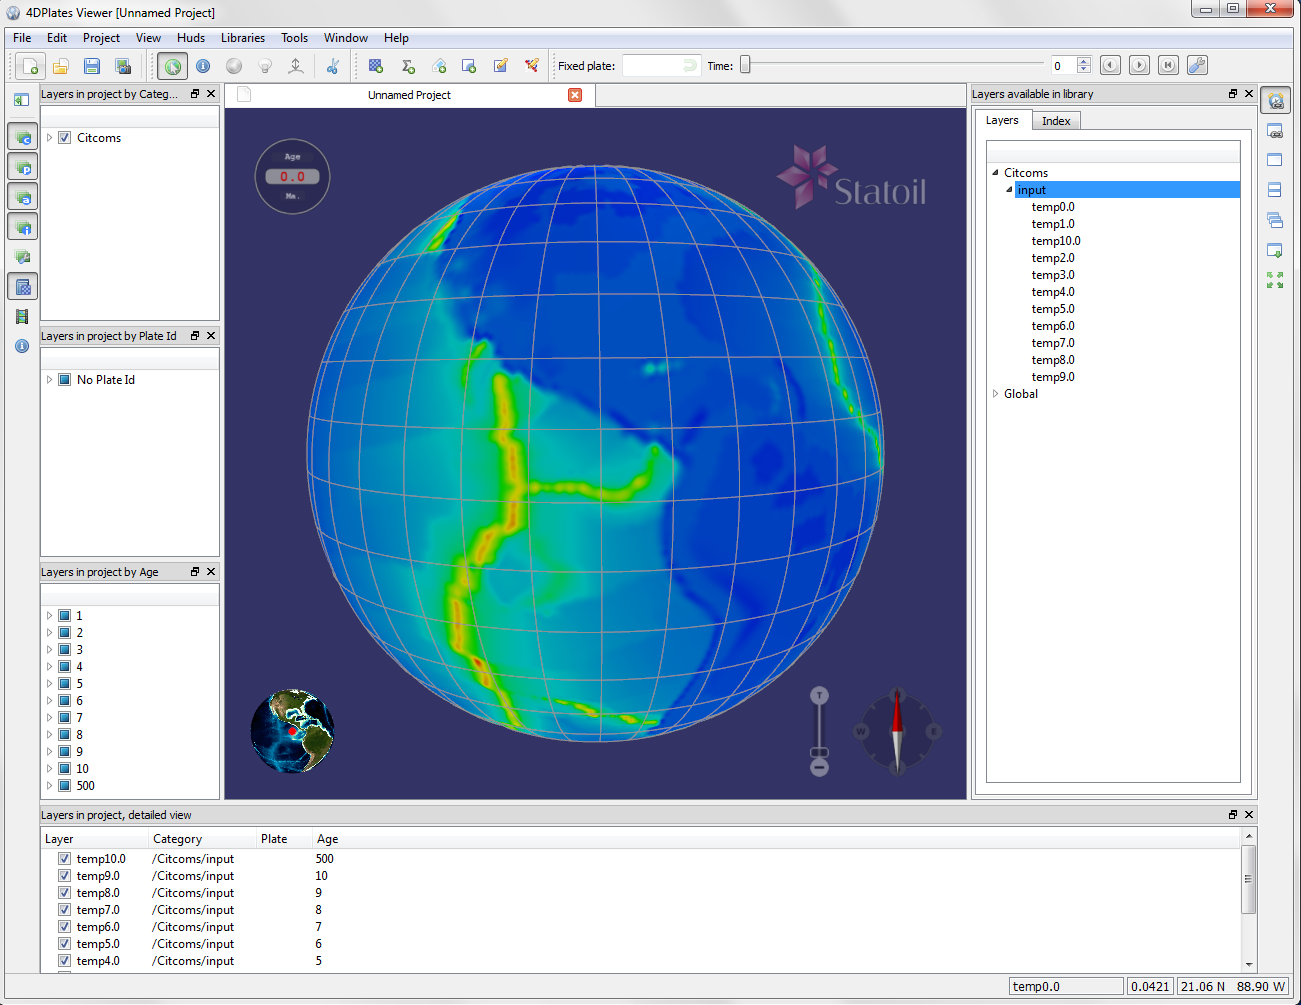
\includegraphics[width=1.0\textwidth]{figs/4DPlates_step2.png}
\caption{Step 2. Drag the entire CitComS case onto the globe to show time-dependant data. }
\label{fig:cont2ps}
\end{figure}

Please see 4DPlates documentation for more information on its tools and features.

\newpage

\bibliographystyle{agu08}
\bibliography{refs}


\appendix
\section{Troubleshooting}
\begin{itemize}
\item Ensure that you have data files for the previous age otherwise CitcomS will exit without providing a helpful error message.  For example, if you start a model at 30 Ma, you must also have data files for 31 Ma.
\end{itemize}

\section{Known bugs}
\begin{itemize}
\item Avoid creating an initial condition using the CitcomS function ``lith\_age\_construct\_tic'' since it is not compatible with the modifications made for the assimilation workflow.  For example, it cannot handle ``no assimilation regions'' and will truncate lithosphere ages according to \verb#lith_age_min# which could cause problems if also using \verb#lith_age_depth_function#.
%\item Lithosphere ages in the `lith' files must be positive or less than the lith\_age\_stencil\_value that is used in the CitcomS .cfg file to define non-stenciled regions.  lith\_age\_min in CitcomS .cfg doesn't actually do anything at the moment but in future we should use it; it was probably disabled to enable us to use lith\_age\_stencil\_value.  This change would make the code more robust, although Create\_history.py already ensures that lithosphere ages are greater than a minimum value.
\end{itemize}




\section{Appendix 1: Summary Table}

\begin{itemize}
\item This table sumarizes the standard test case example files described in this document and used to validate the Geodynamic Framework linking GPlates and CitcomS.

%\item Table 
\scriptsize
\begin{tabular}{ | l | l | }
  \hline \hline \hline
  Section \# & Process and purpose \\
  Programs: & program, script, and module names \\
  Input: & input files and URLs \\
  Output: & input files and URLs \\
  \hline \hline \hline
  Section 0. & ... \\
  programs: & ... \\
  inputs: & ... \\
  outputs: & ... \\
  \hline \hline
  Section 1. & Display a global plate model \\
  Programs: & GPlates  \\
  Inputs: & URL: https://svn.gps.caltech.edu/repos/GPlates/models/ \gplatesmodel \\
  Outputs: & On screen; and in \~{ }/work/GPlates/models/ \gplatesmodel \\
  \hline
.../ & raster\_0.00Ma.png \\

  \hline \hline
  Section 2.1 & Export plate boundary line data \\ 
  Programs: & GPlates  \\
  Inputs: & as Section 1.  \\
  Outputs: & \~{}/work/GPlates/models/ \gplatesmodel /export/*.* \\
  \hline
.../ & topology\_platepolygons\_0.00Ma.xy \\
.../ & topology\_ridge\_transform\_boundaries\_0.00Ma.xy \\
.../ & topology\_slab\_edges\_leading\_0.00Ma.xy \\
.../ & topology\_slab\_edges\_leading\_sL\_0.00Ma.xy \\
.../ & topology\_slab\_edges\_side\_0.00Ma.xy \\
.../ & topology\_slab\_edges\_trench\_0.00Ma.xy \\
.../ & topology\_slab\_polygons\_0.00Ma.xy \\
.../ & topology\_subduction\_boundaries\_0.00Ma.xy \\
.../ & topology\_subduction\_boundaries\_sL\_0.00Ma.xy \\
.../ & topology\_subduction\_boundaries\_sR\_0.00Ma.xy \\

  \hline \hline
  Section 2.2 & Export plate and deforming zone velocity data \\
  Programs: & GPlates \\
  Inputs: & as Section 1. \\
  Outputs: & ~/work/GPlates/models/ \gplatesmodel /export/*.* \\
\hline
.../ & bvel0.0 \\
.../ & bvel0.1 \\
.../ & bvel0.2 \\
.../ & bvel0.3 \\
.../ & bvel0.4 \\
.../ & bvel0.5 \\
.../ & bvel0.6 \\
.../ & bvel0.7 \\
.../ & bvel0.9 \\
.../ & bvel0.10 \\
.../ & bvel0.11 \\

  \hline \hline
  Section 4.1. & ... \\
  Programs: & Create History.py \\
  Inputs: & ... \\
  Outputs: & ... \\

  \hline \hline
  Section 4.2. & ... \\
  Programs: & Create\_History.py \\
  Inputs: & ... \\
  Outputs: & ... \\

  \hline \hline
  Section 4.2. & ... \\
  Programs: & Create\_History.py \\
  Inputs: & ... \\
  Outputs: & ... \\

  \hline \hline

\end{tabular}

%\item Table 
\scriptsize
\begin{tabular}{ | l | l | }

  \hline \hline \hline
  Section 6. & Restarting CitcomS for dynamic topography and total topography \\
  Programs: & restart\_citcoms.py \\
  Inputs: & restart.cfg \\
  Outputs: & A set of secondary CitcomS input .cfg files \\
  \hline \hline \hline

  \hline \hline \hline
  Section N. & ... \\
  Programs: & ... \\
  Inputs: & ... \\
  Outputs: & ... \\
  \hline \hline \hline

\end{tabular}

\end{itemize}
\end{document}
